\chapter{Evaluation and Discussion}
\label{chap:eval}
\chaptermark{Evaluation and Discussion}

\section{Sweep Results}

\subsection{Hyperparameter-Error Correlation Analysis}
Based on our exhaustive hyperparameter sweep, we identified the correlation between hyperparameters and validation performance.

Most of the shared hyperparameters exhibit a \textbf{neutral correlation} with validation performance. These include: 
\texttt{slmerr\_k}, \texttt{batch\_size}, \texttt{train\_prediction\_length}, \texttt{emg\_samples\_per\_frame}, and \texttt{predict\_hidden\_layer\_size}.

However, a few hyperparameters show consistent \textbf{non-neutral correlation} across both architectures:
\begin{itemize}
    \item \texttt{train\_length} and \texttt{l2} exhibit a \textbf{positive correlation} in both CNN and STS setups.
    \item \texttt{poses\_in\_context} shows a \textbf{negative correlation} in both CNN and STS setups.
\end{itemize}

Several hyperparameters exhibit \textbf{disagreement} between the CNN and STS setups, where one model shows a distinct correlation while the other remains largely unaffected. Specifically, 
\texttt{vel\_k} and \texttt{train\_sample\_ratio} show a \textbf{negative correlation} in the CNN setup but fall back to \textbf{neutral} in STS. 
Conversely, \texttt{lr} and \texttt{context\_span} exhibit a \textbf{positive correlation} in STS, while remaining \textbf{neutral} in CNN. 
Similarly, \texttt{accel\_k} and \texttt{synapse\_features} show a \textbf{negative correlation} in STS, but again \textbf{neutral} in CNN. 
This pattern suggests these hyperparameters are more architecture-sensitive and their influence does not generalize across models.

In some cases, the correlation not only differs in strength but in \textit{direction} between architectures. 
Notably, \texttt{train\_patches} exhibits a \textbf{positive correlation} in CNN but a \textbf{negative correlation} in STS. 
Likewise, both \texttt{frames\_per\_window} and \texttt{l1} show a \textbf{negative correlation} in CNN and a \textbf{positive correlation} in STS, further emphasizing divergent optimization behavior.

Interestingly, the hyperparameters allowing train split to grow larger, namely \texttt{train\_length}, \texttt{train\_sample\_ratio} and \texttt{train\_patches}, show a very diverse correlation with the validation metric -- hence a deeper investigation was conducted to evaluate non-linear dependencies. As the result, it was found that the dependency is indeed non-linear neither any monotonic. It appears to be that the optimal range of the interval to train is \textbf{14-18 minutes}, a bigger split harms the prediction results. Such a  investigation imply that the slow-varying drift, subject fatigue, and nonstationary artifacts has a severe affect in a long term sessions, disallowing for a model to keep being effective.

Among the architecture-specific hyperparameters, distinct trends were also observed. 
In the CNN setup, both \texttt{conv\_layer1\_kernels} and \texttt{conv\_layer2\_kernels} exhibited a \textbf{strong positive correlation} with the validation mean landmark error, 
indicating that larger kernel counts may lead to overfitting or excess model capacity. 
In contrast, \texttt{conv\_out\_kernels} demonstrated a \textbf{neutral correlation}, at the same time having low importance metric -- suggesting that model can broadly adopt without overfitting even if having redundant output size.

In the STS setup, all model-specific hyperparameters — namely, 
\texttt{slice\_width}, \texttt{std\_width}, \texttt{mx\_width}, \texttt{std\_stride}, \texttt{slices}, \texttt{patterns}, and \texttt{mx\_stride} — showed consistently \textbf{neutral correlation} 
with model performance. This suggests that while these parameters control the spatial decomposition of input features, they do not critically impact model generalization within the tested range -- indeed the importance metric for all of them is also low, suggesting that either that the default STS can already capture meaningful features good enough or it.

\subsection{Hyperparameter Importance Analysis}
We also identified the parameters whose deviations mostly affect model`s performance.  
The rankings below list these \emph{most sensitive} hyperparameters for each architecture.

\begin{enumerate}
    \item \textbf{STS setup - most sensitive hyperparameters}
    \begin{itemize}
        \item \textbf{muscle\_features}
        \item \textbf{l1}
        \item \textbf{l2}
        \item \textbf{frames\_per\_window}
    \end{itemize}

    \item \textbf{CNN setup - most sensitive hyperparameters}
    \begin{itemize}
        \item \textbf{conv\_layer2\_kernels}
        \item \textbf{l2}
        \item \textbf{train\_sample\_ratio}
        \item \textbf{synapse\_features}
    \end{itemize}
\end{enumerate}

\section{Inter-Subject Exploration and Fit Without EMG}

\subsection{Selected Hyperparameters}

Following the hyperparameter correlation and importance analysis, we picked the following values for the evaluation on the second stage:

{\small
\begin{longtable}{l|c|c}
\captionsetup{justification=centering}
\caption[Hyperparameter Values for STS and CNN]{Hyperparameter values used in STS and CNN setups.} \label{tab:hypers_values} \\
\hline
\textbf{Hyperparameter} & \textbf{STS Value} & \textbf{CNN Value} \\
\hline
\endfirsthead
\multicolumn{3}{@{}l}{\tablename\ \thetable{} -- continued from previous page} \\
\hline
\textbf{Hyperparameter} & \textbf{STS Value} & \textbf{CNN Value} \\
\hline
\endhead
emg\_samples\_per\_frame       & 32           & 32           \\
slmerr\_k                      & 1.0          & 1.0          \\
vel\_k                         & 1.0          & 1.0          \\
accel\_k                       & 10.0         & 10.0         \\
lr                             & 1e-4         & 1e-4         \\
l1                             & 1e-4         & 1e-1         \\
l2                             & 1e-4         & 1e-4         \\
context\_span                  & 512 ms       & 512 ms       \\
poses\_in\_context             & 6            & 6            \\
conv\_layer1\_kernels          & ---          & 32           \\
conv\_layer2\_kernels          & ---          & 32           \\
conv\_out\_kernels             & ---          & 32           \\
synapse\_features              & 512          & 512          \\
muscle\_features               & 32           & 32           \\
predict\_hidden\_layer\_size   & 128          & 128          \\
batch\_size                    & 32           & 32           \\
train\_length                  & 14 min       & 14 min       \\
train\_prediction\_length      & 2 s          & 2 s          \\
train\_patches                 & 20000        & 20000        \\
train\_sample\_ratio           & 0.05         & 0.05         \\
slices                         & 32           & ---          \\
patterns                       & 32           & ---          \\
slice\_width                   & 128 ms       & ---          \\
mx\_width                      & 64 ms        & ---          \\
mx\_stride                     & 60 ms        & ---          \\
std\_width                     & 64 ms        & ---          \\
std\_stride                    & 60 ms        & ---          \\
\hline
\end{longtable}
}

\paragraph{Quality}
Both STS and CNN versions observed to produce visually correct results while inferring on a test split -- a separate interval not included neither in train nor in validation split. Numerically the quality can be quantified with landmark error progression. There is the error plot of the STS version trained and evaluated on a EMG2Pose session:

\begin{figure}[H]
    \centering
    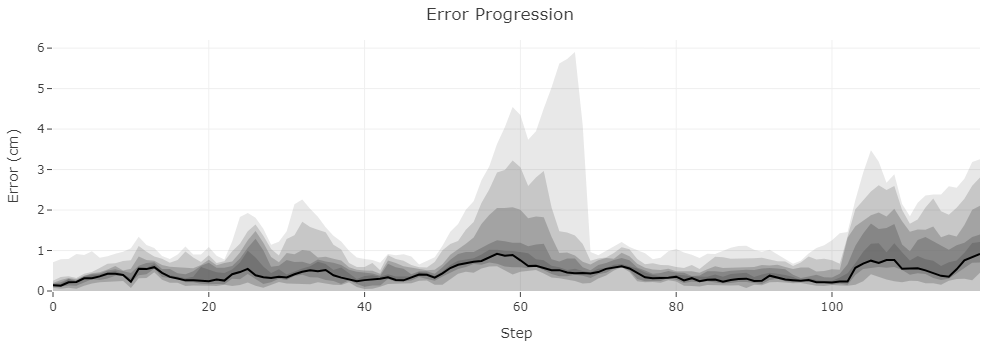
\includegraphics[width=1.0\textwidth]{error_progression.png}
    \caption{A Inference Error Progression.}
    \label{fig:error_progression}
\end{figure}

Overall the validation metrics achieved by both models across training individually on all sessions are presented in the table:

\textbf{TODO: table STS/CNN | EMG/NoEMG on ours/emg2pose}
% TODO: to table STS/CNN | EMG/No EMG
% - Mean landmark error of 18+-5mm (TODO) is nearly equivalent for both the models
% - Mean landmark error of 18+-5mm (TODO) for the models using CNN fit without EMG
% - Mean landmark error of 18+-5mm (TODO) for the models using STS fit without EMG

Both models perform equally no under having or not having emg information. Notably at the perspective of fit without emg both models perform nearly the same too. This clue is indicating that the shared part of both models, namely the final layers that are directly fed with the poses are responsible for that notion of fit without emg.

Nevertheless the presence of fit without emg indicates that the hand motion present in the dataset itself is predictable enough for model to overfit to it and the problem cannot be spotted on the validation metric. As a corollary, for our datasets of random motion, a greater difference in the validation metric between the models trained with and without EMG information is observed.

\paragraph{Model Size}
STS appears to be more expensive in terms of parameters while having the same quality. In case of the benchmarked models, STS weights \textbf{3.2 MB} with \textbf{840 K} parameters, while CNN version is just acquiring \textbf{1 MB} with \textbf{250 K} parameters.

\paragraph{Training and Inference Time}
Because of the size of the models, while benchmarking the Phase II, mean time to train a STS model is observed to be about \textbf{1.5 hours}. On the other hand, mean time to train a CNN version is measured to be about \textbf{1 hour}. -- This indicates that STS is faster to execute under the same number of parameters, but the fact that it required more parameters to achieve the same quality outbalanced the training time.

Similar situation appears at the inference time. Where CNN model is able to perform \textbf{1200 predictions per second} on a \textbf{AMD Ryzen 7 7735HS} CPU. While for a bigger STS model prediction rate is about \textbf{900 predictions per second} on the same hardware.